\usetikzlibrary{arrows,decorations.markings,decorations.pathmorphing,backgrounds,positioning,fit,petri}

\begin{figure}
 \centering
 \scalebox{0.82}{
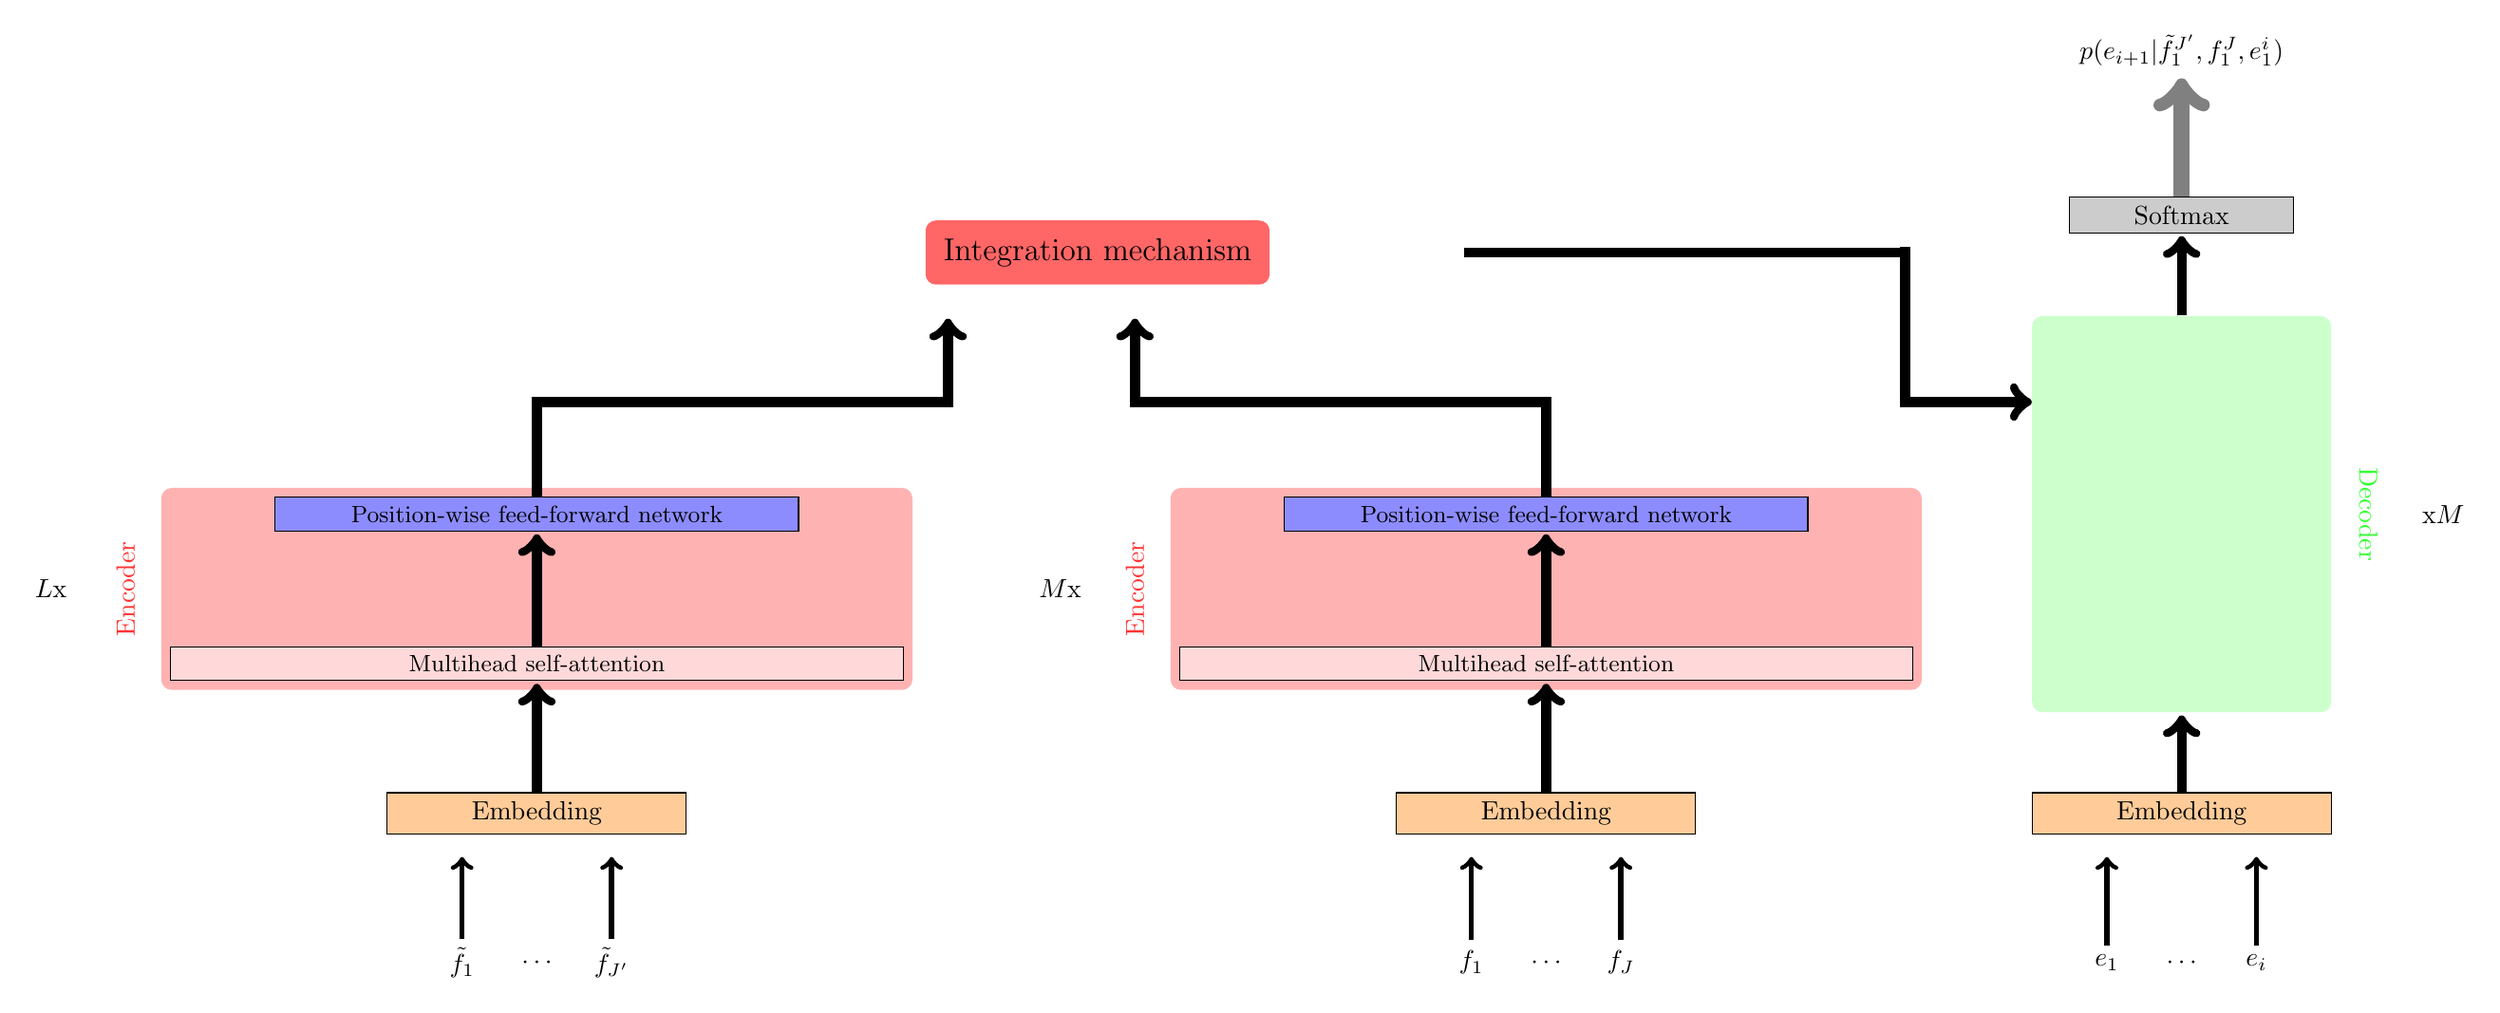
\begin{tikzpicture}[shorten >=1pt, auto, node distance=3cm, ultra thick,
   node_style/.style={circle,draw=blue,fill=blue!20!,font=\sffamily\Large\bfseries},
   edge_style/.style={draw=black}]
    \tikzstyle{embedding}=[rectangle, draw=black, thin, fill=orange!40, minimum width=4cm];
    \tikzstyle{self_att_layer} = [rectangle, draw=black, thin, fill=pink!60, minimum width=9.8cm];
    \tikzstyle{att_layer} = [rectangle, draw=black, thin, fill=pink!20, minimum width=11.66cm];
    \tikzstyle{ffn} = [rectangle, draw=black, thin, fill=blue!45, minimum width=7cm];
    \tikzstyle{softmax} = [rectangle, draw=black, thin, fill=black!20, minimum width=3cm];
    
    \tikzstyle{decoder_box} = [rectangle,fill=green!20,rounded corners,minimum width=4cm, minimum height=5.3cm];
    
    \tikzstyle{n}=[edge_style,line width=2pt];
    \tikzstyle{m}=[edge_style,very thick,line width=3.75pt];
    
    
    \tikzstyle{every pin edge}=[<-,shorten <=1pt];
    \tikzstyle{neuron}=[circle,fill=black!25,minimum size=17pt,inner sep=0pt]    
    \tikzstyle{input neuron}=[neuron, fill=green!50];
    \tikzstyle{output neuron}=[neuron, fill=red!50];
    \tikzstyle{block}=[rectangle, draw=black, thin];
    \tikzstyle{input} = [text centered]
    \tikzstyle{attention} = [block, text width=3em, text centered, minimum height=2.2em]
    \tikzstyle{rnn} = [block, text width=1.5em, text centered, fill=white, minimum width=1.5em,
                                minimum height=2em, rounded corners=.5em]
    \tikzstyle{rnn_block} = [block, line width=1pt, inner sep=0.2em,minimum width=3em,
                                minimum height=5.2em, fill=gray!50]
    \tikzstyle{decoder_block} = [block, line width=1pt, inner sep=0.2em,minimum width=13em,
                                minimum height=2.5em, fill=gray!10, draw=black!30]
    \tikzstyle{cross}=[circle, draw=black, thin, path picture={\draw[black]
        (path picture bounding box.south) -- 
        (path picture bounding box.north) (path picture bounding box.east) -- 
        (path picture bounding box.west)
        (path picture bounding box.north) (path picture bounding box.west) --
        (path picture bounding box.east);}]
    
    \tikzstyle{bl}=[edge_style, bend left]
    \tikzstyle{br}=[edge_style, bend right]
    \tikzstyle{attedge}=[edge_style, draw=blue]
    \tikzstyle{alpha}=[edge_style, draw=red, densely dotted]
    \tikzstyle{attinput}=[edge_style, draw=SeaGreen, thick, dashed]
    
    
    %%%% Variables
    \newcommand\XSEP{-12.5}
    \newcommand\XENC{1}
    \newcommand\XDEC{9.5}
    
  
    %%%%%%%%%%%%%%%%%%%%%%%%%%%%%%%%%%%%%%%%%%%%%%
    % Input ENCODER
    %%%%%%%%%%%%%%%%%%%%%%%%%%%%%%%%%%%%%%%%%%%%%%
    %% previous target sentence
%    \node[input] (f1_p) at (-4,-2){$\tilde{f}_1$};
%    \node[input] (fdots_p) at (-3,-2){$\cdots$};
%    \node[input] (fJ_p) at (-2,-2){$\tilde{f}_{J'}$};
%    
%    \node[input] (fbreak) at (0,-2){\footnotesize $<$BREAK$>$};
        
    %% current source sentence
    \node[input] (f1) at (0,-2){$f_1$};
    \node[input] (fdots) at (\XENC,-2){$\cdots$};
    \node[input] (fJ) at (2,-2){$f_{J}$};
                                
    % Embedding
    \node[embedding] (embedd_enc) at (\XENC,0){Embedding};
    
%    \draw[->, n] (f1_p) -- (-4,-0.55);
%    \draw[->, n] (fJ_p) -- (-2,-0.55);
%    \draw[->, n] (fbreak) -- (0,-0.55);
    \draw[->, n] (f1) -- (0,-0.55);
    \draw[->, n] (fJ) -- (2,-0.55);
    %%%%%%%%%%%%%%%%%%%%%%%%%%%%%%%%%%%%%%%%%%%%%%
    %% ENCODER %%%%%%%%%%%%%%%%%%%%%%%%%%%%%%%%%%%
    %%%%%%%%%%%%%%%%%%%%%%%%%%%%%%%%%%%%%%%%%%%%%%
    %% Self Attention
    \node[self_att_layer] (self_att_enc) at (\XENC,2){\small Multihead self-attention};
    \draw[->, m] (embedd_enc) -- (self_att_enc);
    
    %% FFNs
    \node[ffn] (ffn_enc) at (\XENC,4){\small Position-wise feed-forward network};
    \draw[->, m] (self_att_enc) -- (ffn_enc);
    
    \begin{pgfonlayer}{background}
    \node [fill=red!30, rounded corners,fit=(self_att_enc) (ffn_enc)] {};
    \end{pgfonlayer}
    \node[rotate=90,red!80] (encoder_text) at (-4.5,3){Encoder};
    \node (encoder_layers) at (-5.5,3){$M$x};
    
    %%%%%%%%%%%%%%%%%%%%%%%%%%%%%%%%%%%%%%%%%%%%%%
    %% SEPERATE ENCODER %%%%%%%%%%%%%%%%%%%%%%%%%%
    %%%%%%%%%%%%%%%%%%%%%%%%%%%%%%%%%%%%%%%%%%%%%%
    
    % sep. Embedding
    \node[embedding] (embedd_enc_sep) at (\XSEP,0){Embedding};
    
    %% previous source sentence
    \node[input] (f1_p) at (-13.5,-2){$\tilde{f}_1$};
    \node[input] (fdots_p) at (\XSEP,-2){$\cdots$};
    \node[input] (fJ_p) at (-11.5,-2){$\tilde{f}_{J'}$};
    
    \draw[->, n] (f1_p) -- (-13.5,-0.55);
    \draw[->, n] (fJ_p) -- (-11.5,-0.55);
    
    
    %% Self Attention
    \node[self_att_layer] (self_att_enc_sep) at (\XSEP,2){\small Multihead self-attention};
    \draw[->, m] (embedd_enc_sep) -- (self_att_enc_sep);
    
    %% FFNs
    \node[ffn] (ffn_enc_sep) at (\XSEP,4){\small Position-wise feed-forward network};
    \draw[->, m] (self_att_enc_sep) -- (ffn_enc_sep);
    
    \begin{pgfonlayer}{background}
    \node [fill=red!30, rounded corners,fit=(self_att_enc_sep) (ffn_enc_sep)] {};
    \end{pgfonlayer}
    \node[rotate=90,red!80] (encoder_text) at (-18,3){Encoder};
    \node (encoder_layers) at (-19,3){$L$x};
    
    % Integration Mechanism
    \node (integration) at (-5,7.5) {\large Integration mechanism};
    
    \begin{pgfonlayer}{background}
    \node [fill=red!60, rounded corners,fit=(integration)] {};
    \end{pgfonlayer}
    
    % seperate encoder to integration
    \draw[-, m] (ffn_enc_sep.north) -- (\XSEP,5.5);
    \draw[-, m] (-12.57,5.5) -- (-7,5.5);
    \draw[->, m] (-7,5.43) -- (-7,6.65);
    
    % encoder to integration
    \draw[-, m] (ffn_enc.north) -- (\XENC,5.5);
    \draw[-, m] (1.07,5.5) -- (-4.5,5.5);
    \draw[->, m] (-4.5,5.43) -- (-4.5,6.65);
    
    \draw[-, m] (-0.1,7.5) -- (5.8,7.5);
    \draw[-, m] (5.8,7.57) -- (5.8,5.5);
    \draw[->, m] (5.73,5.5) -- (7.53,5.5);
    
    
    
    %%%%%%%%%%%%%%%%%%%%%%%%%%%%%%%%%%%%%%%%%%%%%%%%%%%%%%%%%%%%%%%%%%
    % Input DECODER
    %%%%%%%%%%%%%%%%%%%%%%%%%%%%%%%%%%%%%%%%%%%%%%
    %% previous target sentence
%    \node[input] (e1_p) at (9,-2){$\tilde{e}_1$};
%    \node[input] (edots_p) at (10,-2){$\cdots$};
%    \node[input] (eJ_p) at (11,-2){$\tilde{e}_{I'}$};
%    
%    \node[input] (ebreak) at (13,-2){\footnotesize $<$BREAK$>$};
    
    %% current target sentence
    \node[input] (e1) at (8.5,-2){$e_1$};
    \node[input] (edots) at (\XDEC,-2){$\cdots$};
    \node[input] (eJ) at (10.5,-2){$e_{i}$};
    % Embedding
    \node[embedding] (embedd_dec) at (\XDEC,0){Embedding};
%    \draw[->, n] (e1_p) -- (9,-0.55);
%    \draw[->, n] (eJ_p) -- (11,-0.55);
%    \draw[->, n] (ebreak) -- (13,-0.55);
    \draw[->, n] (e1) -- (8.5,-0.55);
    \draw[->, n] (eJ) -- (10.5,-0.55);
    
    %%%%%%%%%%%%%%%%%%%%%%%%%%%%%%%%%%%%%%%%%%%%%%
    %% DECODER %%%%%%%%%%%%%%%%%%%%%%%%%%%%%%%%%%%
    %%%%%%%%%%%%%%%%%%%%%%%%%%%%%%%%%%%%%%%%%%%%%%
    %% Self Attention
%    \node[self_att_layer] (self_att_dec) at (13,2){Masked multihead self-attention};
    
    %% Cross Attention
%    \node[att_layer] (att_dec) at (13,4){Multihead cross-attention};
%    \draw[->, m] (self_att_dec) -- (att_dec);
%    \draw[->, m] (ffn_enc.east) -- (att_dec.west);
    
    %% FFNs
%    \node[ffn] (ffn_dec) at (13,6){Position-wise feed-forward network};
%    \draw[->, m] (att_dec) -- (ffn_dec);
    
%    \begin{pgfonlayer}{background}
%    \node [fill=green!20, rounded corners,fit=(self_att_dec) (att_dec) (ffn_dec)] {};
%    \end{pgfonlayer}

    \node[decoder_box] (decoder_box) at (\XDEC,4) {};
    
    \draw[->, m] (embedd_dec) -- (decoder_box.south);
%    \draw[->, m] (ffn_enc.east) -- (decoder_box.west);
    
    
    \node[rotate=-90,green!80] (decoder_text) at (12,4){Decoder};
    \node (decoder_layers) at (13,4){x$M$};
    
    %% Output softmax
    \node[softmax] (softmax) at (\XDEC,8){Softmax};
    \draw[->, m] (decoder_box) -- (softmax);
    
    \node (output) at (\XDEC,10.2){$p(e_{i+1}|\tilde{f}_1^{J'}, f_1^J,e_1^i)$};
    \draw[->,black!50, line width=6pt] (softmax) -- (output);
\end{tikzpicture}}
%\caption{Transformer Architecture with concatenated sentences as additional context-information. Here we consider one previous context-sentence on the source ($\tilde{f}_1^{J'}$) and target ($\tilde{e}_1^{I'}$) side. The $<$BREAK$>$ token seperates the sentences.}
\label{fig:concat_baseline_multi}
\end{figure}
